\documentclass[fleqn,10pt]{wlscirep}
\usepackage[utf8]{inputenc}
\usepackage[T1]{fontenc}
\usepackage{lineno}
\usepackage{xurl}
\usepackage{numprint}
\usepackage[colorinlistoftodos,prependcaption,textsize=tiny]{todonotes}
\usepackage{listings}
%%For better lookin Listings
\usepackage{xcolor}
\usepackage[inkscapelatex=false, inkscapearea=page]{svg}

\definecolor{codegreen}{rgb}{0,0.6,0}
\definecolor{codegray}{rgb}{0.5,0.5,0.5}
\definecolor{codepurple}{rgb}{0.58,0,0.82}

\lstdefinestyle{rdf}{
    commentstyle=\color{codegreen},
    keywordstyle=\color{magenta},
    numberstyle=\tiny\color{codegray},
    stringstyle=\color{codepurple},
    basicstyle=\ttfamily\footnotesize,
    breakatwhitespace=false,         
    breaklines=true,                 
    captionpos=b,                    
    keepspaces=true,                                  
    showspaces=false,                
    showstringspaces=false,
    showtabs=false,                  
    tabsize=2
}

\lstset{style=rdf}


\linenumbers

\title{Handout: Sicherung der Korrektheit von durch LLMs erzeugtem Code}

\author{Istvan J. Mocsy}


\begin{abstract}
Die Nutzung von Large Language Models(LLMs) zur Codeerzeugung ist in den letzten Jahren deutlich gestiegen. Bei der Nutzung von diesem erzeugtem Code kann und sollte man sich die Frage stellen: Ist dieser Code wirklich funktional korrekt? Im von diesem Handout begleitendem Vortrag wird die Testbenchmark HumanEval vorgestellt, welche eine Lösung im Bereich Korrektheitsüberprüfung von durch LLMs erzeugtem Code anbietet. Gleichzeitig soll eine Überischt der Entstehung der LLM Codex gegeben werden, welche sich auf Codeerzeugung funktional Korrekter Programme spezialisiert. Im Abschluss wird EvalPlus vorgestellt, ein Framework welches bestehende Benchmark-Datensätze optimiert und mit welchem eine verbesserte Variante von HumanEval erzeugt wird.
\end{abstract}
\begin{document}

\flushbottom
\maketitle
%  Click the title above to edit the author information and abstract

\thispagestyle{empty}
\section*{HumanEval}
HumanEval ist ein Framework zum Benchmarking von durch LLMs erzeugtem Code. Im Kern liegt hier ein Datensatz, welcher die Programmierprobleme abbildet und zu diesen eine Musterimplementierung(Ground-Truth) sowie Unit Tests bereitstellt. Ein Programmierproblem besteht immer aus der Signatur der gewünschten Funktion, eine Beschreibung im Docstring-Format und Beispiele für Inputs sowie gewünschten Output, wie in Abbildung 1 dargestellt. Insgesamt stehen 164 Programmierprobleme zur verfügung mit durchschnittlich 7,7 Tests pro Problem.\cite{chen2021evaluating}
    \begin{figure}
        \centering
        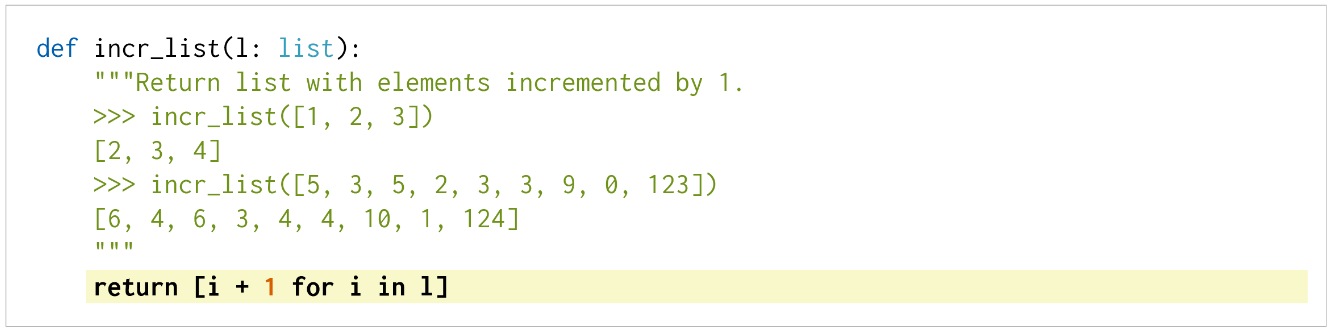
\includegraphics[width=0.8\paperwidth]{image/humanevalproblem.png}
        \caption{HumanEval Problemstellung bestehend aus Signatur, Docstring und Beispiel In/Outputs.           Ebenfalls wird ein erfolgreich generiertes Codesample gezeigt.\cite{chen2021evaluating}}
    \end{figure}
\section*{Codex}
Codex ist ein feineingestelltes GPT-3 Modell, welches mit bis zu 12B Parametern erzeugt wurde. Zum Training wurden Github-Repositories in der Sprache Python verwendet, gefiltert nach Kriterien wie weniger als 1MB Dateigröße, maximale Zeilenanzahl von 1000, Ausschluss von automatisch generierten Repositories. Es wurden weitere Varianten erzeugt. Codex-S wurde mit Trainingsdaten höherer Qualität trainiert, welche aus Coding-Challenges und Repos mit Continuous Integration(CI) gesammelt wurden. Insgesamt wurden 50.000 Programmierprobleme als Trainingsdaten verwendet.\cite{chen2021evaluating}
\section*{EvalPlus}
EvalPlus ist ein Framework, welches bestehende Frameworks zum Benchmarking von LLM-Code verbessert. Während EvalPlus generalisiert konzipiert wurde, wird sich im Vortrag auf die Verbesserung von HumanEval zu HumanEval+ fokussiert. 

\begin{figure}
    \centering
    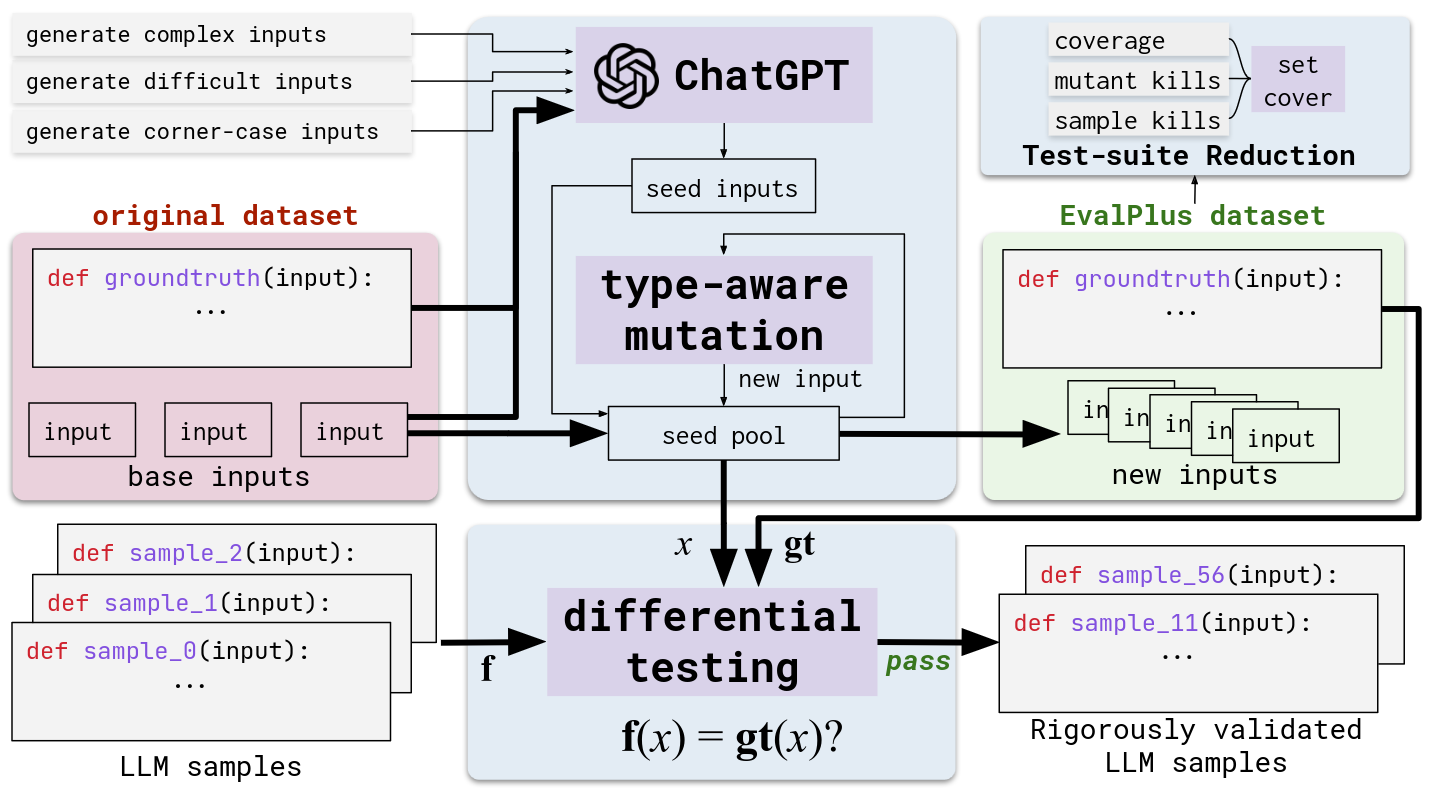
\includegraphics[width=0.8\paperwidth]{image/overviewEplus.png}
    \caption{Übersicht zum EvalPlus framework\cite{liu2024your}}
\end{figure}
EvalPlus bedient sich an den Programmierproblemen des zugrunde liegenden Frameworks und speichert die Testinputs in einem Seedpool. Ferner werden die Originalinputs sowie die Ground-Truth Implementierung mit der Anweisung weitere Inputs, insbesondere für schwere Fälle oder Randfälle, zu generieren an ChatGTP gesendet. Nach Bereinigung werden diese dem Seedpool hinzugefügt und dieser wird einer type-aware Mutation unterzogen, welcher je nach Datentyp neue Inputs nach Mutationsregeln erzeugt( z.B. x +/- 1 für Integer). Aus diesem Datensatz wird ebenfalls ein reduzierter Testfall-Datensatz erzeugt. Im Framework ist auch eine Testsuite enthalten, welche mit dem verbesserten Datensatz über diffential testing die LLM Samples validiert. Das Gesamtmodell wird in Abbildung 2 dargestellt.

\begin{figure}
    \centering
    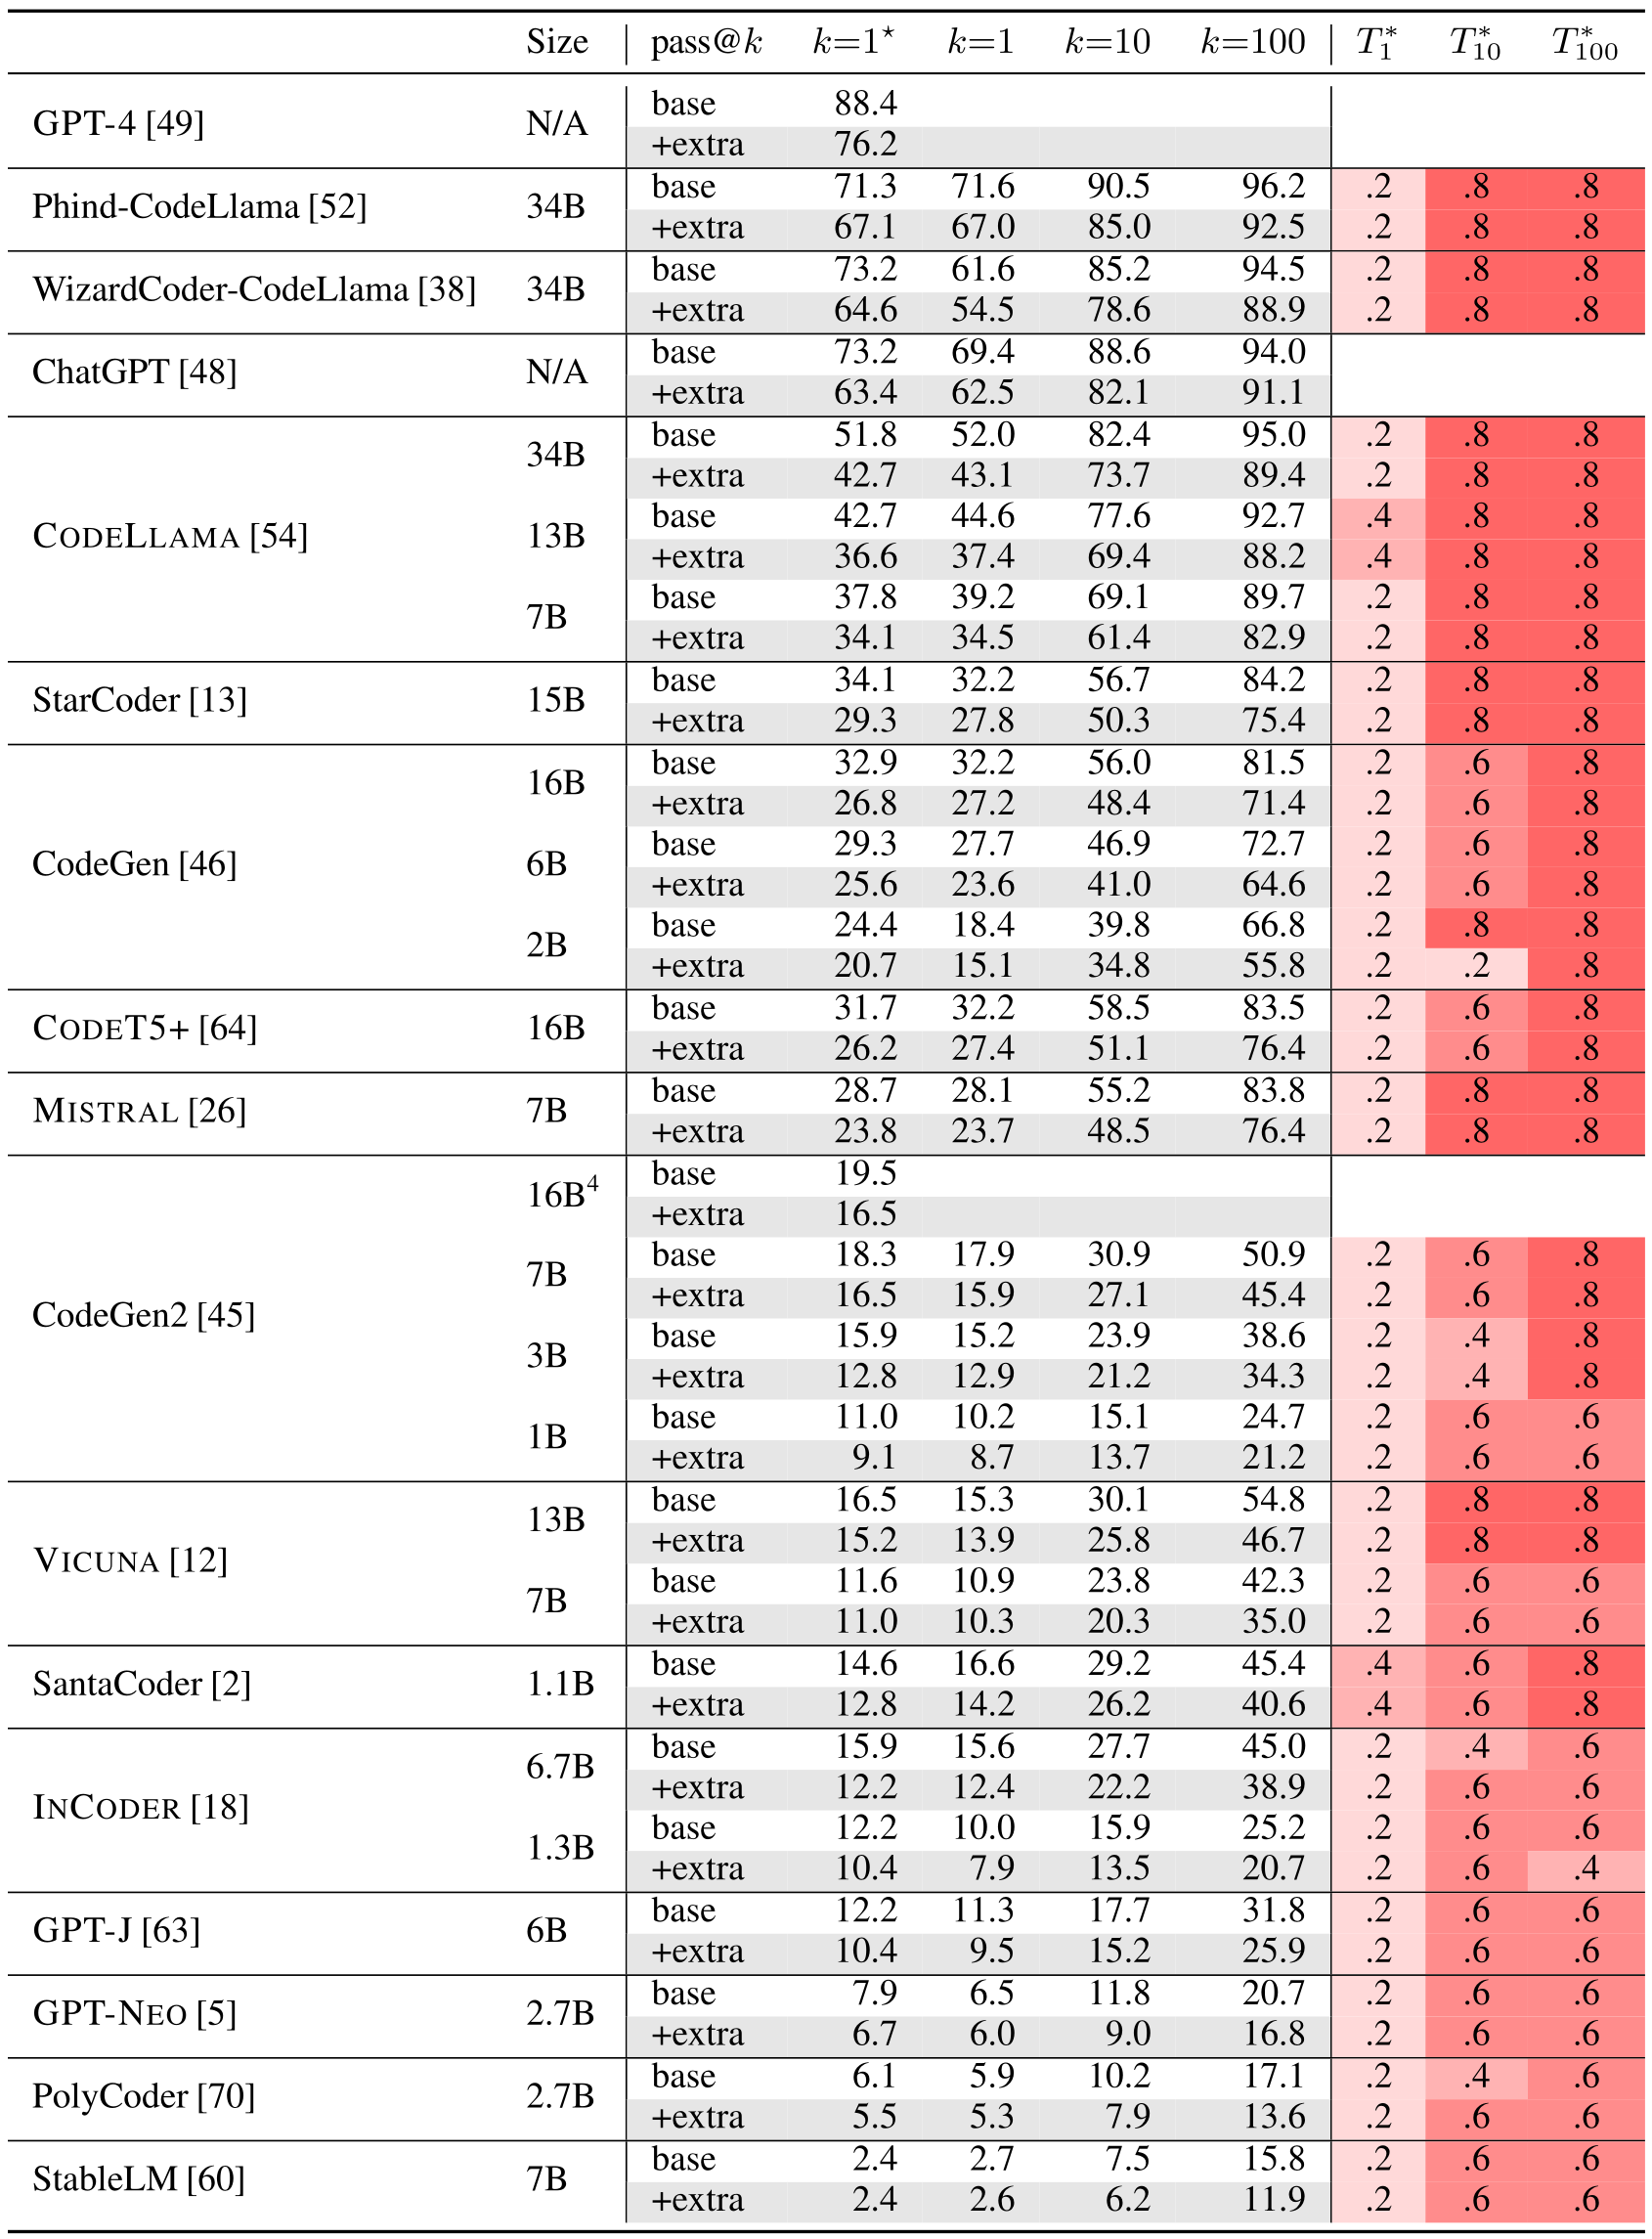
\includegraphics[width=0.8\paperwidth]{image/resultshumaneval+full.png}
    \caption{Vollständge Ergebnistabelle der LLMs im Vergleich zwischen HumanEval und HumanEval+\cite{liu2024your}}
\end{figure}
In der Ergebnistabelle aus Abbildung 3 ist zu sehen, dass mit dem verbesserten Testframework HumanEval+ bei allen LLMs ein Abstieg des pass@k zu beobachten ist. 



\bibliography{sample}
\end{document}